% !TEX spellcheck = en
%% document class file for the preparation of a paper
%% for the International Conference ICCAS 2007
%% global option 'fleqn' ensures equations flush left.
%% set '10pt' and 'twocolumn' options.

\documentclass[fleqn,10pt,twocolumn]{ICCAS2012}

%%%%%%% set heading and page number heare %%%%%%%%%%
%\setcounter{page}{101}
\begin{document}

\title{High Degree of Freedom Humanoid Robot Error Mitigation}

\author{Kevin Lynch${}^{1}$, Daniel M. Lofaro${}^{2}$, and Paul Oh${}^{3}$ }

\affils{  	${}^{1}$Department of Computer Science, \\
		${}^{2}$Department of Electrical and Computer Engineering, \\
		${}^{3}$Department of Mechanical Engineering,\\
Drexel University, Philadelphia, PA, USA\\
EMAIL: kml43@drexel.edu, dml46@drexel.edu, paul@coe.drexel.edu\\ 
        }
\thanks{*This project was supported by the Drexel Autonomous Systems Lab (DASL) and by a National Science Foundation - Partnerships for International Research and Education grant (\#0730206).}% <-this % stops a space
%\thanks{ \noindent
%   This paper is supported by my funding agencies.
%  }
\abstract{
This work shows a plan for error state determination, diagnosis, and mitigation using autonomic computing tools and tecniques on the Hubo robot. An $n$-dimensional geometric enclosure is constructed from periodic measurements of the robot's normal operating state. Similar hulls will be constructed for unique faults encountered during runtime. A mapping of these faults to applicable mitigations will be dynamically constructed and will aid in mitigation selection. The successful application of the mitigation will bring the robot back to a safe operating state.
}

\keywords{
    High Degree of Freedom Humanoid Robot Error Mitigation
}

\maketitle

%-----------------------------------------------------------------------
\section{Introduction}
Electro-mechanical systems eneviatiaibly fail during use.  Failors during opperation typically cause system haults.  This is particuralaly hazerdous to robots that require feedback to ballance such as biped humanoid robots.  For biped humanoids these errors typically include, but are not limited to, actuator failure due to over torque or loss of zero-moment-point (ZMP) \cite{zmp35} causing a robot fall or colapse.  This is exceptionally harmful to adult size humanoid robots due to their weight.  This paper focuses on way of automatically detecting when a failure is about to occure and choosing the proper mitigation technique. 

Current methods of mitigation of ZMP loss for biped humanoids been invistigated by Kiyoshi Fujiwara et al. \cite{4115653}.  These methods involve finding an optiomal falling trajectory that reduces the instanous force of the robot at impact by creating multiple impact stages\cite{4399327}.  This method was fully tested on an HRP-2FX (HRP-2P surragate) and partiailly on an HRP-2P.  This work did not include a method of determining a falling state, it is assummed that a fall is in progress.  Additional work on detecting a fall and reducing fall damage has been shown by Kunihiro Ogata et al.\cite{4755950}.  An active shok-reducing motion reduces the impact damage by following the center of gravity (COG) and attempting to keep it close to the ZMP support polygon.  The falling state is determined when the predicted ZMP departs from the support polygon. This method was tested on a miniture humanoid robot.  Addiotonal work on determining a fall state using machine learning techniques\cite{4813885}.

\section{Methodology}



\subsubsection{Mitigation Analysis}
\label{ssub:mitigation_analysis}
The effectiveness of different mitigations has been analyzed on faults injected into two different systems typically used as benchmark applications in the software engineering community, RUBiS\footnote{http://rubis.ow2.org/} and Hadoop\footnote{http://hadoop.apache.org/}. RUBiS is a web application auction site running on the Apache Tomcat\footnote{http://tomcat.apache.org/} web server and serves page requests to hundreds of concurrently simulated clients. Hadoop is a distributed task manager that processes gigabytes of data across multiple nodes. We injected faults into both systems, the virtual machines they are running on, as well as the hosts managing the virtual machines. The faults consumed either processor, memory, disk, database, or network resources in the respective components. We applied generic mitigations that restarted various components, migrated the components to new hosts or virtual machines, or did nothing. The effectiveness of each fault-mitigation pair was analyzed on each system to generate a mapping of faults to mitigations. Using this knowledge, if a fault is later encountered, the best mitigation can be applied with a high chance of success. If a particular mitigation cannot be applied in that instance, then the next best mitigation may be selected, and so forth.



% When an anomaly occurs, multiple mitigations may be triggered at once. For instance, if a hardware failure is detected on a host, all process should be migrated to another machine and diagnostic utilities should be run on the machine.

A naive observer would expect the two systems to have nearly identical fault-mitigation mappings. However, in our testing on software based systems the generated mappings varied greatly in the effectiveness of the mitigations on a particular fault.  RUBiS is a typical web application that receives requests from clients and processes results returned from a database. Little processing is being done by RUBiS or its host machine, so even though a processor intensive fault may be using up many cycles in the process or the host, there is no noticeable effect on the request processing rate. As a result, any mitigation applied would result in more down time than if no mitigation were to be applied. Unlike RUBiS, Hadoop is much more processor intensive. Any host level fault that is slowing down the system will adversely affect the completion time for the task. Another major difference is that RUBiS, like many other request driven systems, can easily be restarted to temporarily address fault symptoms, while restarting Hadoop typically means losing already processed results.  We expect similar results when applying this method to the complex electro-mechanical platforms Jaemi Hubo/Hubo2+.

The generated fault-mitigation mappings for the two systems offer insight into their respective natures. On the surface, both software systems operate like typical servers, waiting for requests or tasks, and processing them in a timely fashion. However, the way the requests are handled results in faults manifesting in different ways. Even though a fault may be detected, the obvious mitigation is not always the best. This approach to mitigation analysis, will offer valuable insight into the true effectiveness of mitigations when faults occur in Hubo.




\subsection{none}












The robot that will be used is the adult-size humanoid robot Jaemi Hubo, see Fig.~\ref{fig:huboSch}.  Jaemi Hubo is a high gain position controlled device.  Each actuator is fed a reference position and is able to feed back the actual position, the current through the actuator, and the actuator status (enabled or disabled).  Each actuator has an over current automatic disable routine.  When this routine is executed the motor control is deactivated but feedback of the actual position is still enabled.  This routine was determined to be the cause of Jaemi Hubo's ankle failure.

\begin{figure}[thpb]
  \centering
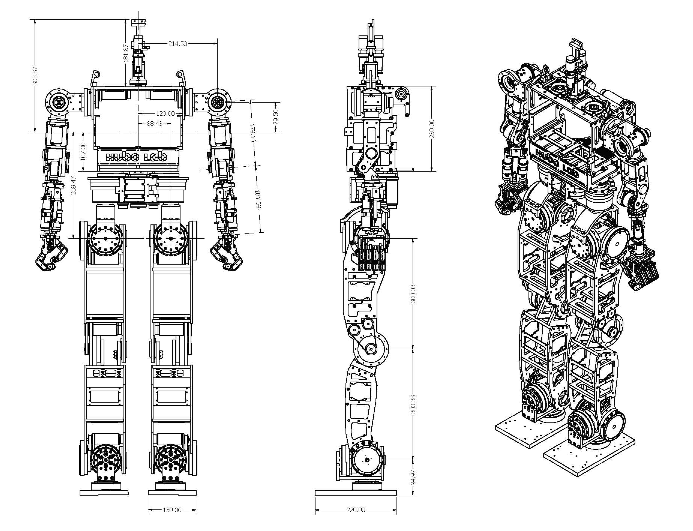
\includegraphics[width=1.0\columnwidth]{./pix/huboSch.png}
  \caption{Jaemi Hubo: 130cm tall 45kg (with battery and protective shell) 40 degree of freedom, high gain position controlled adult-size humanoid robot }
  \label{fig:huboSch}
\end{figure}

Real time constraints. Difficult to simulate faults with robot.

Collect data from all metrics, and construct convex hull for normal state. If metric is not useful, it will not affect hull (metric is independent of other metrics).

Faults include over torque of actuators, loss of zero-moment-point, over-current disable

Mitigations include: restart actuator, reduce current (disable noncritical actuator?), rebalance (shift position in various ways, move body, make sure feet are on ground, etc.) 


%%%%%%%%%%%%%%%%% BIBLIOGRAPHY IN THE LaTeX file !!!!! %%%%%%%%%%%%%%%%%%%%%%
%%---------------------------------------------------------------------------%%
%
%\begin{thebibliography}{99}


%\bibliographystyle{plain}
%\bibliography{mit}

\bibliographystyle{IEEEtran}
%\bibliographystyle{plain}
\bibliography{mit}{}


%\end{thebibliography}

%
%%--------------------------------------------------------------------%%

\end{document}
